% \section {Design} <cross>copy & paste</cross> well modify & revise it; justify the changes
\section{Design}
\subsection{Anticipated components of the system}
\par\noindent
The main partition of the system was a software that enables to simulate
and visualise each interaction before convergence (or terminate). The project
would also attempt to explore one or more protocol to check their internal
status after finishing the software.

\par\noindent
The simulator would allow users to choose from a set of well-defined protocol and
specify the parameters for these protocol (e.g. number of agents participating).
The simulator would allow users to easily extend their own protocol though writing
structured few lines of code, an the extension should be as easy as possible.

\par\noindent
The system expected to have a ability to simulate some variations (which at
least includes the network constructor \cite{MS16a} and terminating grid network constructor in 2D \cite{Mi17})
of the original protocol according the protocol and dynamically visualise how process (nodes) transfer for each interaction.

\par\noindent
The interface provided would be a desktop application running on Java Virtual Machine Platform.
A web interface was desirable but would not be guaranteed to deliver.

\paragraph{Modification from original design}
\begin{itemize}
  \item The original design mentioned it could include "a configuration parser to
  enable user define a protocol from configuration files" finally replaced by a set of
  well-defined set of protocol and a programmable interface. This is because the
  original design requires a design and implementation of Domain Specific Language (DSL),
  and a parser of this kind of "new language", which is a large work load and might be
  infeasible to finish all of them
  during the project period. This might be done in the following development plan
  after finishing the project itself.
\end{itemize}

\subsection{Data structure, algorithms and Pseudo-code for key method}
\subsubsection{Adjacency List}
\par\noindent
For some specific kinds of models, specifically ,the network constructor, a data
structure to maintain a undirected graph $G$ formed from current configuration $C$ is required. In other words, it requires to maintain
a group of status of ”active” edges. It aims to construct ”shapes”
and there are some status for the edge $uv$ in between any nodes (processors) $u$
and $v$ in the population.

\par\noindent
To make it, an adjacency list would be used to record the connections associated
with each



\paragraph{Modification from original design}
\subsubsection{Graph}
\paragraph{Modification from original design}
\subsubsection{Terminating grid network constructor: Check acceptable configuration \& Handle rotation}  %mention BFS
\paragraph{Modification from original design}
\subsection{Interaction (Sequence) Design}
\begin{figure}[H]
\begin{center}
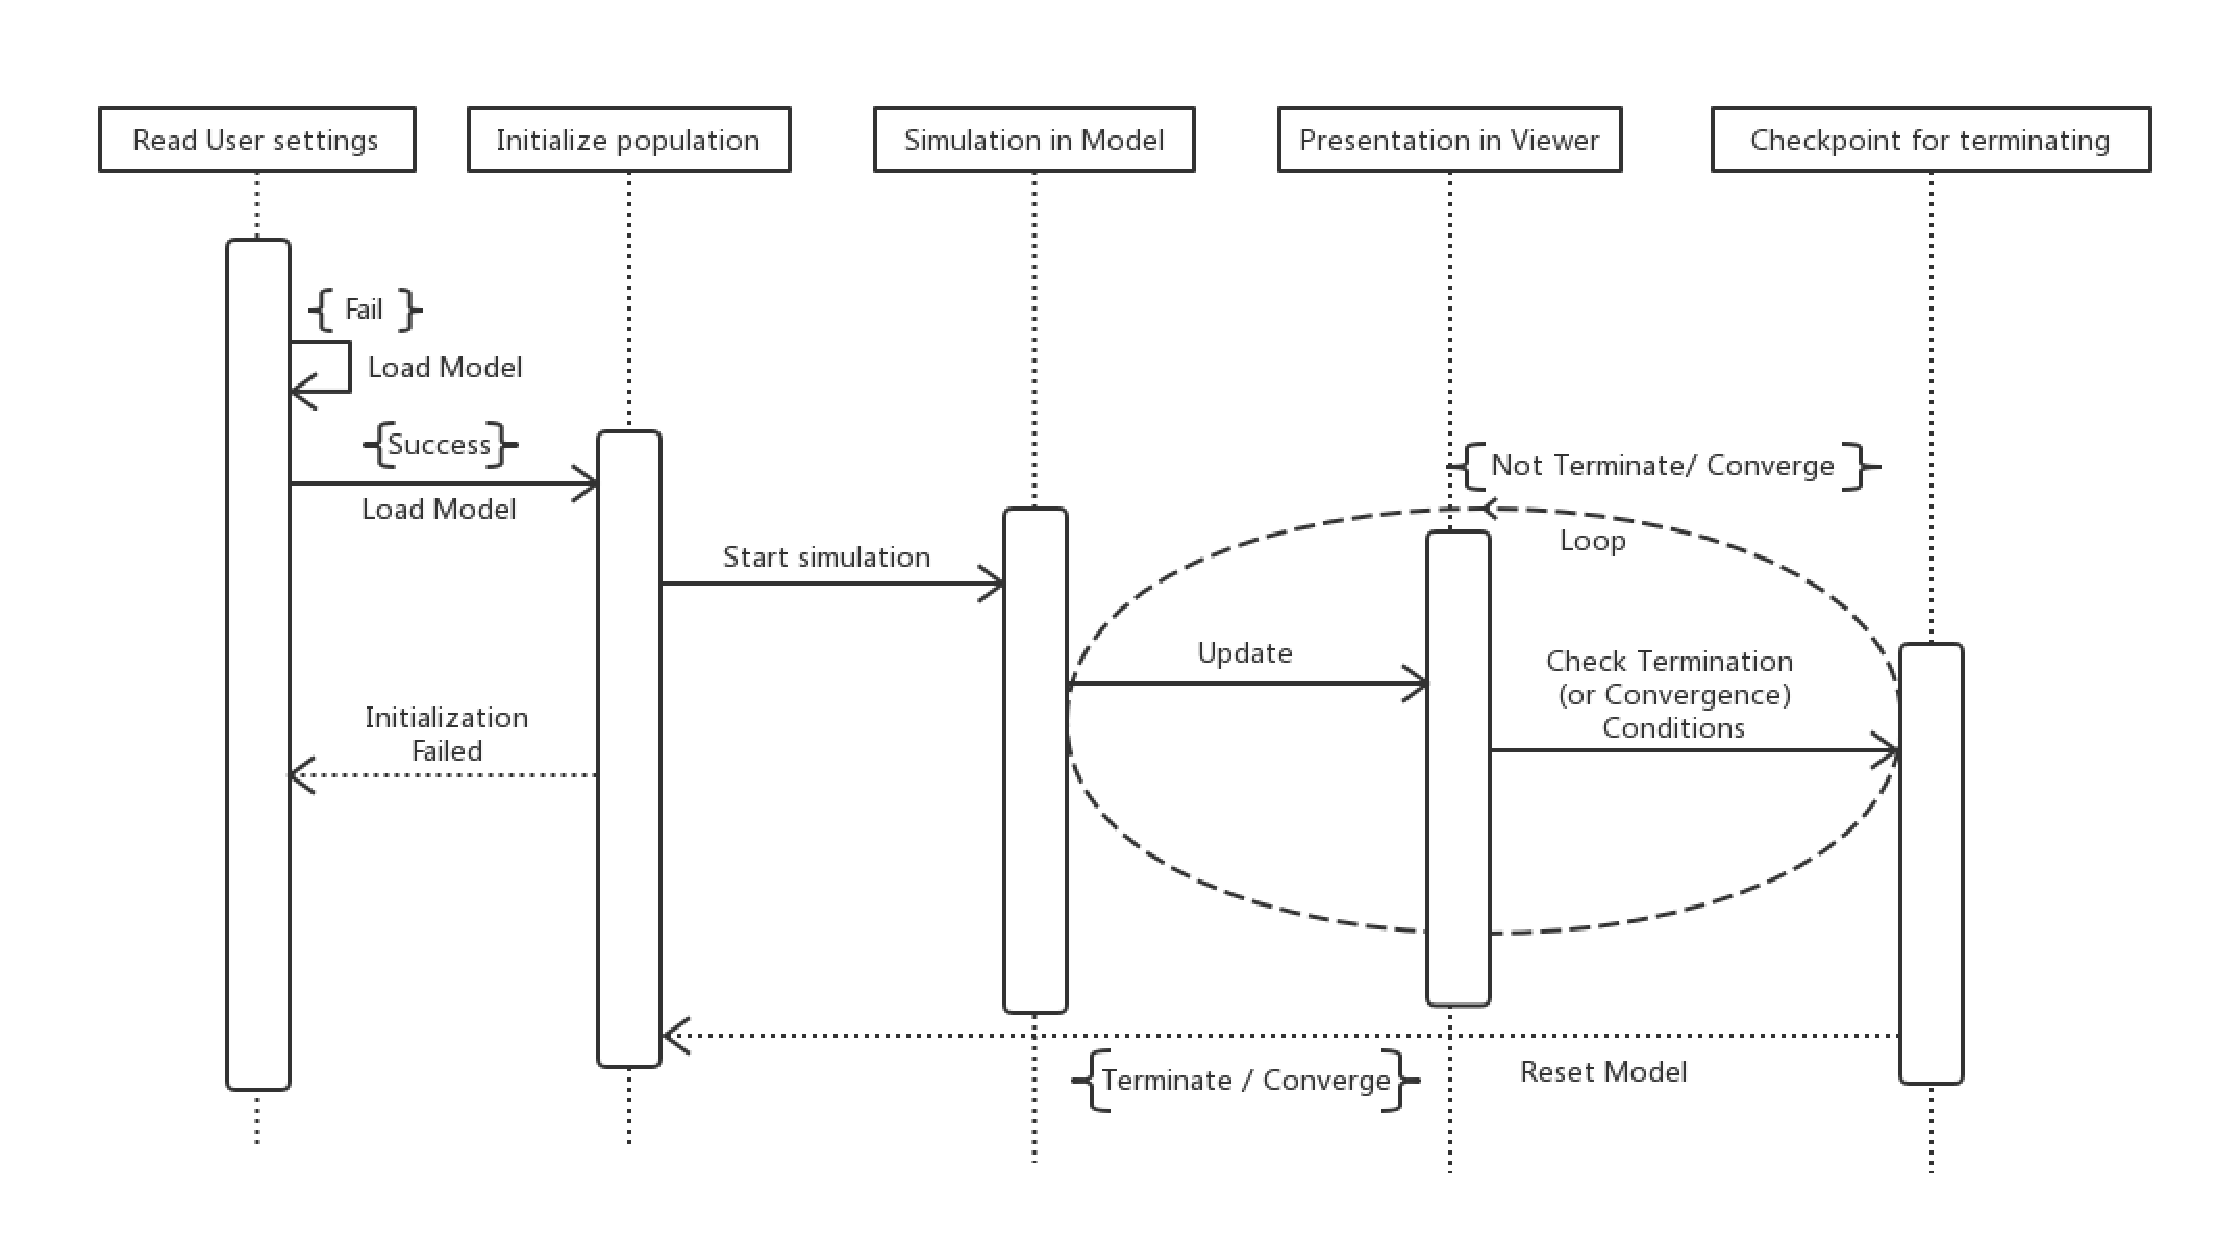
\includegraphics[width =\textwidth]{context/diagram/interaction.pdf}
\caption{Interaction Design Diagram}
\label{interactionG}
\end{center}
\end{figure}

\par\noindent
The figure \ref{interactionG} illustrates the entire interaction process of the
simulator. Initially, the user select one protocol from a set of well-defined
protocols and then select a set of parameters required such as how many nodes to
be included in the simulation, the initial status distribution for nodes and so forth.
Then the user click the "Apply settings button" to apply the model settings. before
applying the model, the program itself would check whether all parameters are
well-defined, i.e. locating in the value range they should be. If they are, the software
would load the model otherwise it will reject this particular request from user and
allow user to repeat its (possibly) another setting.

\par\noindent
After the program successfully loaded a model, the user can press the "Start simulation"
button to start a simulation. A simulation contains multiple rounds. For each round,
the model executes interaction simulation under the control of scheduler specified in one
of parameters mentioned before and then the model would update the states of elements
 in viewer to show the what happened in the model itself. Following that, the model would
 check whether it reaches a configuration that should stop the simulation. A stop can be caused
 by user's temporarily interruption (pause) or the fact that the number of consistent accumulation of
 inefficient interactions overwhelms a pre-configured parameters defined in the model (which indicates
 a terminating or convergence with a high possibility). If the model does not detect a stop,
 it will continue the "interact - update - checking stop" process as a loop. Once it detect a
 stop, the software will return to state of waiting for starting of a simulation process
 (while the model would keep its internal states and user can build an another new model under this situation).

 \paragraph{Modification from original design}
The current design removed a step of sequence in original sequence design called "Initialize scheduler", which located after "Initialize population" step.
the "Initialize scheduler" process had been integrated into "Initialize population" because
the scheduler partition does not necessarily separated from the population and can be treated as a partition of a "population" in concept.

\subsection{UI Interface Design}
\begin{figure}[H]
\begin{center}
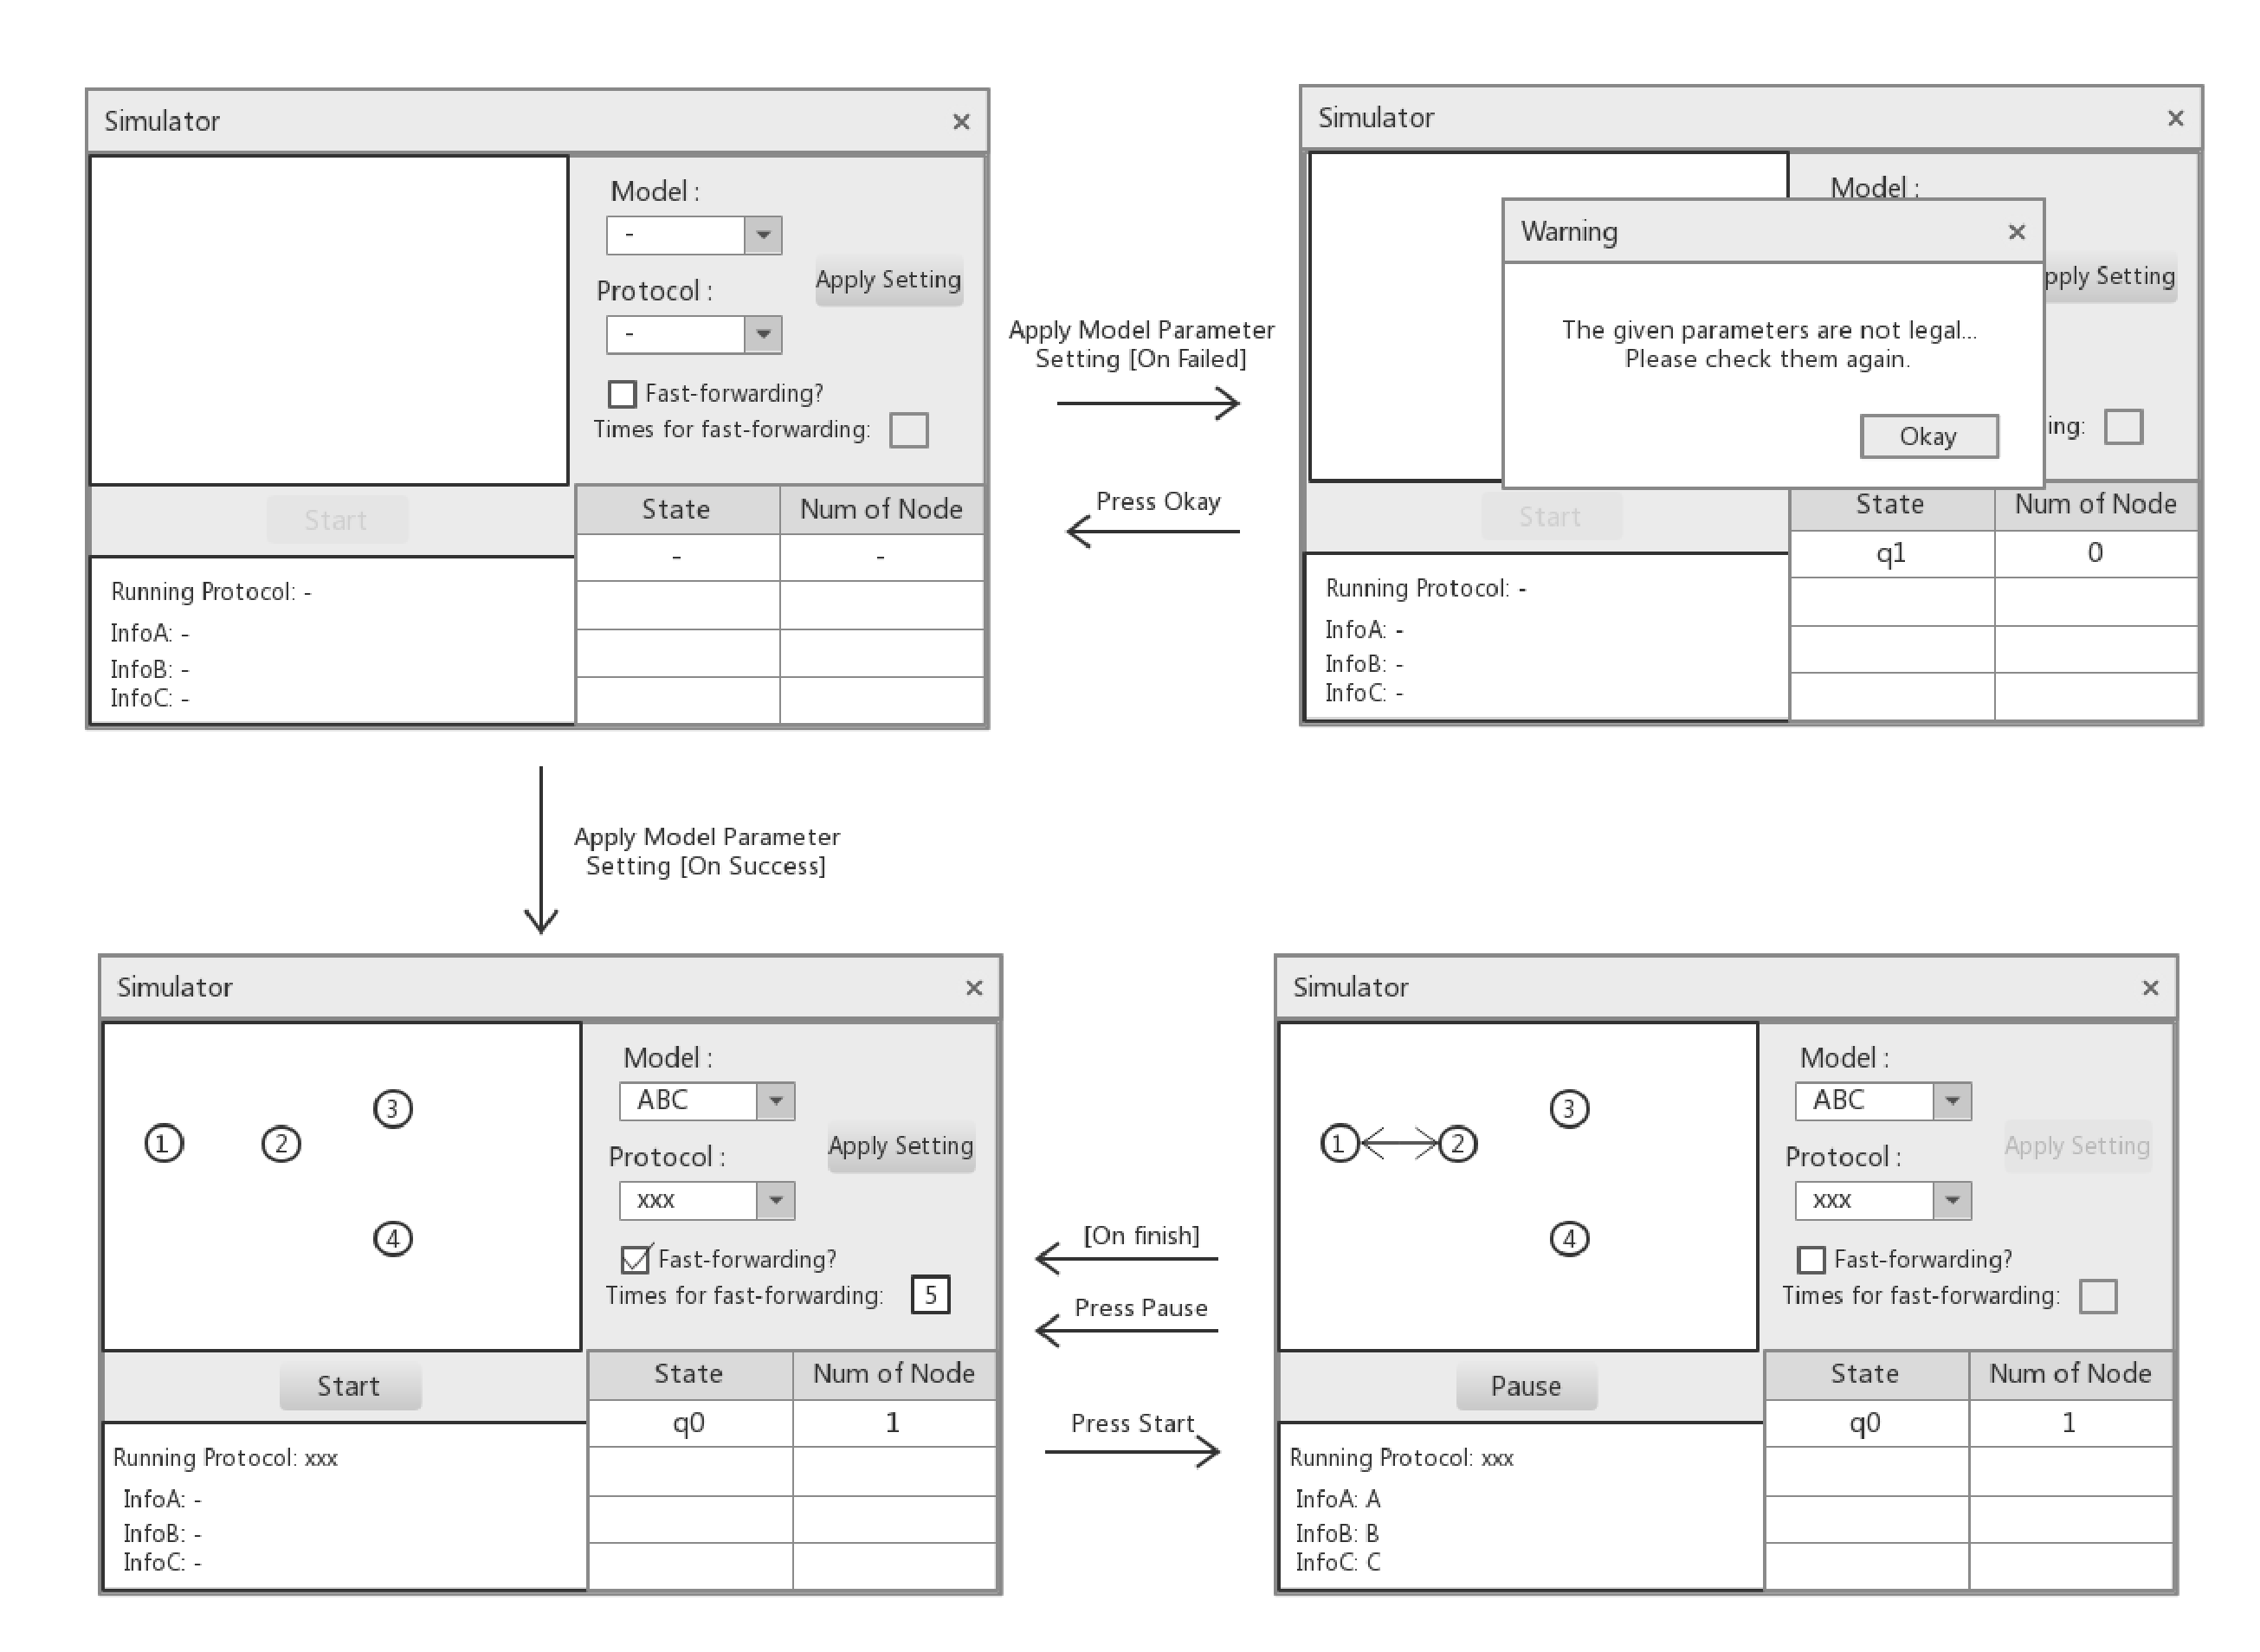
\includegraphics[width =\textwidth]{context/diagram/interface.pdf}
\caption{Interaction Design Diagram}
\label{intefaceG}
\end{center}
\end{figure}

\paragraph{Modification from original design}
The UI was redesigned entirely. This is because the original design built on the assumption
that the users load their settings for some population from domain specification language (DSL) codes residing in
some files. The DSL is infeasible to be finished due to the limited time of implementation.
Hence, the design would allow user to set their population through the UI containing a set of well-defined
protocols and would allow the users to write their own extensional protocol through few lines of codes.
As the functionality changes, the UI removed the functionality entrance for loading files from disk and
added some options to allow user setting the parameters of a protocol. 
